\subsection{RisingWave}

RisingWave merupakan \textit{cloud-native streaming database}. Setelah menghubungkan sumber \textit{stream}, pengguna dapat membuat \textit{query} analisis dengan mendefinisikan \textit{materialized view}, yang diperbarui secara inkremental pada RisingWave \textit{streaming engine} \parencite{risingwave}.

Berikut adalah keuntungan RisingWave:

\begin{enumerate}
    \item Mudah dipelajari karena mengembangkan sintaks yang dimiliki PostgreSQL.
    \item Mudah dioperasikan dan memiliki kebutuhan \textit{resource} yang lebih rendah karena ditulis dalam bahasa sistem Rust.
    \item Mendukung berbagai sumber data dan mampu mengirimkan (\textit{sink}) data ke dalam berbagai sumber, seperti mengambil data dari Apache Kafka lalu hasilnya dikirim ke ClickHouse. RisingWave mendukung integrasi dengan PostgreSQL CDC dan Apache Kafka sebagai \textit{source} dan \textit{sink}.
    \item Menjamin konsistensi pada \textit{materialized view} dengan konsistensi berbasiskan \textit{snapshot}.
\end{enumerate}

\begin{figure}[ht]
    \centering
    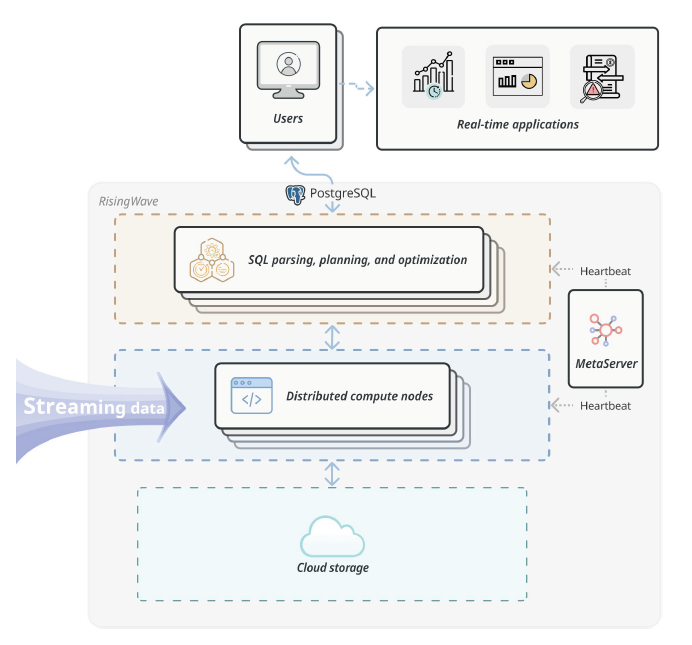
\includegraphics[width=0.8\textwidth]{resources/chapter-2/risingwave.png}
    \caption{\textit{RisingWave Architecture \parencite{risingwave}}}
    \label{fig:risingwave-architecture}
\end{figure}

\textit{Compute nodes} pada RisingWave terdiri atas \textit{batch engine} dan \textit{streaming engine}. \textit{Batch engine} meliputi \textit{query execution engine} dan \textit{exchange service} untuk menukar data antar \textit{compute nodes}. \textit{Streaming engine} dibangun atas model aktor pada pemrograman konkuren. \textit{Engine} ini berinteraksi langsung dengan \textit{frontend} dan melayani \textit{stream data}. Selain itu, terdapat \textit{meta service} yang berperan sebagai layanan sentral untuk menyimpan metadata seperti \textit{state} kluster, katalog sistem, keanggotaan kluster, dan lain-lain \parencite{risingwave}.